% Options for packages loaded elsewhere
\PassOptionsToPackage{unicode}{hyperref}
\PassOptionsToPackage{hyphens}{url}
%
\documentclass[
]{article}
\usepackage{amsmath,amssymb}
\usepackage{iftex}
\ifPDFTeX
  \usepackage[T1]{fontenc}
  \usepackage[utf8]{inputenc}
  \usepackage{textcomp} % provide euro and other symbols
\else % if luatex or xetex
  \usepackage{unicode-math} % this also loads fontspec
  \defaultfontfeatures{Scale=MatchLowercase}
  \defaultfontfeatures[\rmfamily]{Ligatures=TeX,Scale=1}
\fi
\usepackage{lmodern}
\ifPDFTeX\else
  % xetex/luatex font selection
\fi
% Use upquote if available, for straight quotes in verbatim environments
\IfFileExists{upquote.sty}{\usepackage{upquote}}{}
\IfFileExists{microtype.sty}{% use microtype if available
  \usepackage[]{microtype}
  \UseMicrotypeSet[protrusion]{basicmath} % disable protrusion for tt fonts
}{}
\makeatletter
\@ifundefined{KOMAClassName}{% if non-KOMA class
  \IfFileExists{parskip.sty}{%
    \usepackage{parskip}
  }{% else
    \setlength{\parindent}{0pt}
    \setlength{\parskip}{6pt plus 2pt minus 1pt}}
}{% if KOMA class
  \KOMAoptions{parskip=half}}
\makeatother
\usepackage{xcolor}
\usepackage[margin=1in]{geometry}
\usepackage{graphicx}
\makeatletter
\def\maxwidth{\ifdim\Gin@nat@width>\linewidth\linewidth\else\Gin@nat@width\fi}
\def\maxheight{\ifdim\Gin@nat@height>\textheight\textheight\else\Gin@nat@height\fi}
\makeatother
% Scale images if necessary, so that they will not overflow the page
% margins by default, and it is still possible to overwrite the defaults
% using explicit options in \includegraphics[width, height, ...]{}
\setkeys{Gin}{width=\maxwidth,height=\maxheight,keepaspectratio}
% Set default figure placement to htbp
\makeatletter
\def\fps@figure{htbp}
\makeatother
\setlength{\emergencystretch}{3em} % prevent overfull lines
\providecommand{\tightlist}{%
  \setlength{\itemsep}{0pt}\setlength{\parskip}{0pt}}
\setcounter{secnumdepth}{-\maxdimen} % remove section numbering
\usepackage{booktabs}
\usepackage{longtable}
\usepackage{array}
\usepackage{multirow}
\usepackage{wrapfig}
\usepackage{float}
\usepackage{colortbl}
\usepackage{pdflscape}
\usepackage{tabu}
\usepackage{threeparttable}
\usepackage{threeparttablex}
\usepackage[normalem]{ulem}
\usepackage{makecell}
\usepackage{xcolor}
\ifLuaTeX
  \usepackage{selnolig}  % disable illegal ligatures
\fi
\usepackage{bookmark}
\IfFileExists{xurl.sty}{\usepackage{xurl}}{} % add URL line breaks if available
\urlstyle{same}
\hypersetup{
  pdftitle={HCR demo},
  pdfauthor={K. Holsman},
  hidelinks,
  pdfcreator={LaTeX via pandoc}}

\title{HCR demo}
\author{K. Holsman}
\date{1/31/2023}

\begin{document}
\maketitle

{
\setcounter{tocdepth}{3}
\tableofcontents
}
\textbf{Overview}

During ACLIM phase 2 (2019-2022), modelers evaluated a suite of Harvest
Control Scenarios (1-5), in 2025 we added two addition HCRs to the set.
Below is a list of those standardized harvest control rules and the
equations used to derive the curves.

ABC+HCR 1: Status quo\\
ABC+HCR 2: Lagged recovery to estimate emergency relief financing
needs\\
ABC+HCR 3: Long-term resilience (stronger reserve) \(F_{target}\)\\
ABC+HCR 4: CE informed sloping rate, e.g., MHW category alpha\\
ABC+HCR 5: climate sensitivity reserve (buffer shocks)\\
ABC+HCR 6: MHW slope + climate sensitivity reserve (buffer shocks)\\
ABC+HCR 6: Recruit per spawner biomass variability adjusted HCR based on
analyses by Spencer et al.~in prep

\section{ABC+HCR 1: Status quo}\label{abchcr-1-status-quo}

This is the basic sloping harvest control rule for groundfish in the
EBS. There is a B20\% cut-off for SSL (Atka, pollock, P. cod).
\(F_{ABC_{max}}\) is the HCR adjusted F rate that corresponds to ABC.
The Tier three approach is to set the slope of the sloping HCR to
\(\alpha = 0.05\) and \(B_{lim} = 0\) and \(B_{target} = B_{40\%}\) or
\(B_{target} = 0.4B_{100\%}\) (i.e., 40\% of unfished biomass
\(B_{100\%}\), as an MSY proxy) for most species except
\(B_{lim} = B_{20\%}\) for pollock and Pacific cod.

Eq. 1 \[F_{ABC_{max}} = \begin{array}{ll}  
 F_{ABC} &~~~~~~~~ \frac{B_y}{B_{target}}>1 \\  
 F_{ABC}((\frac{B_y}{B_{target}}-\alpha)/(1-\alpha)) &~~~~~~~~ \frac{B_y}{B_{target}} < 1 \leq B_{lim} \\  
 0 &~~~~~~~~ \frac{B_y}{B_{target}} < B_{lim}  
 \end{array}\]

\begin{figure}
\centering
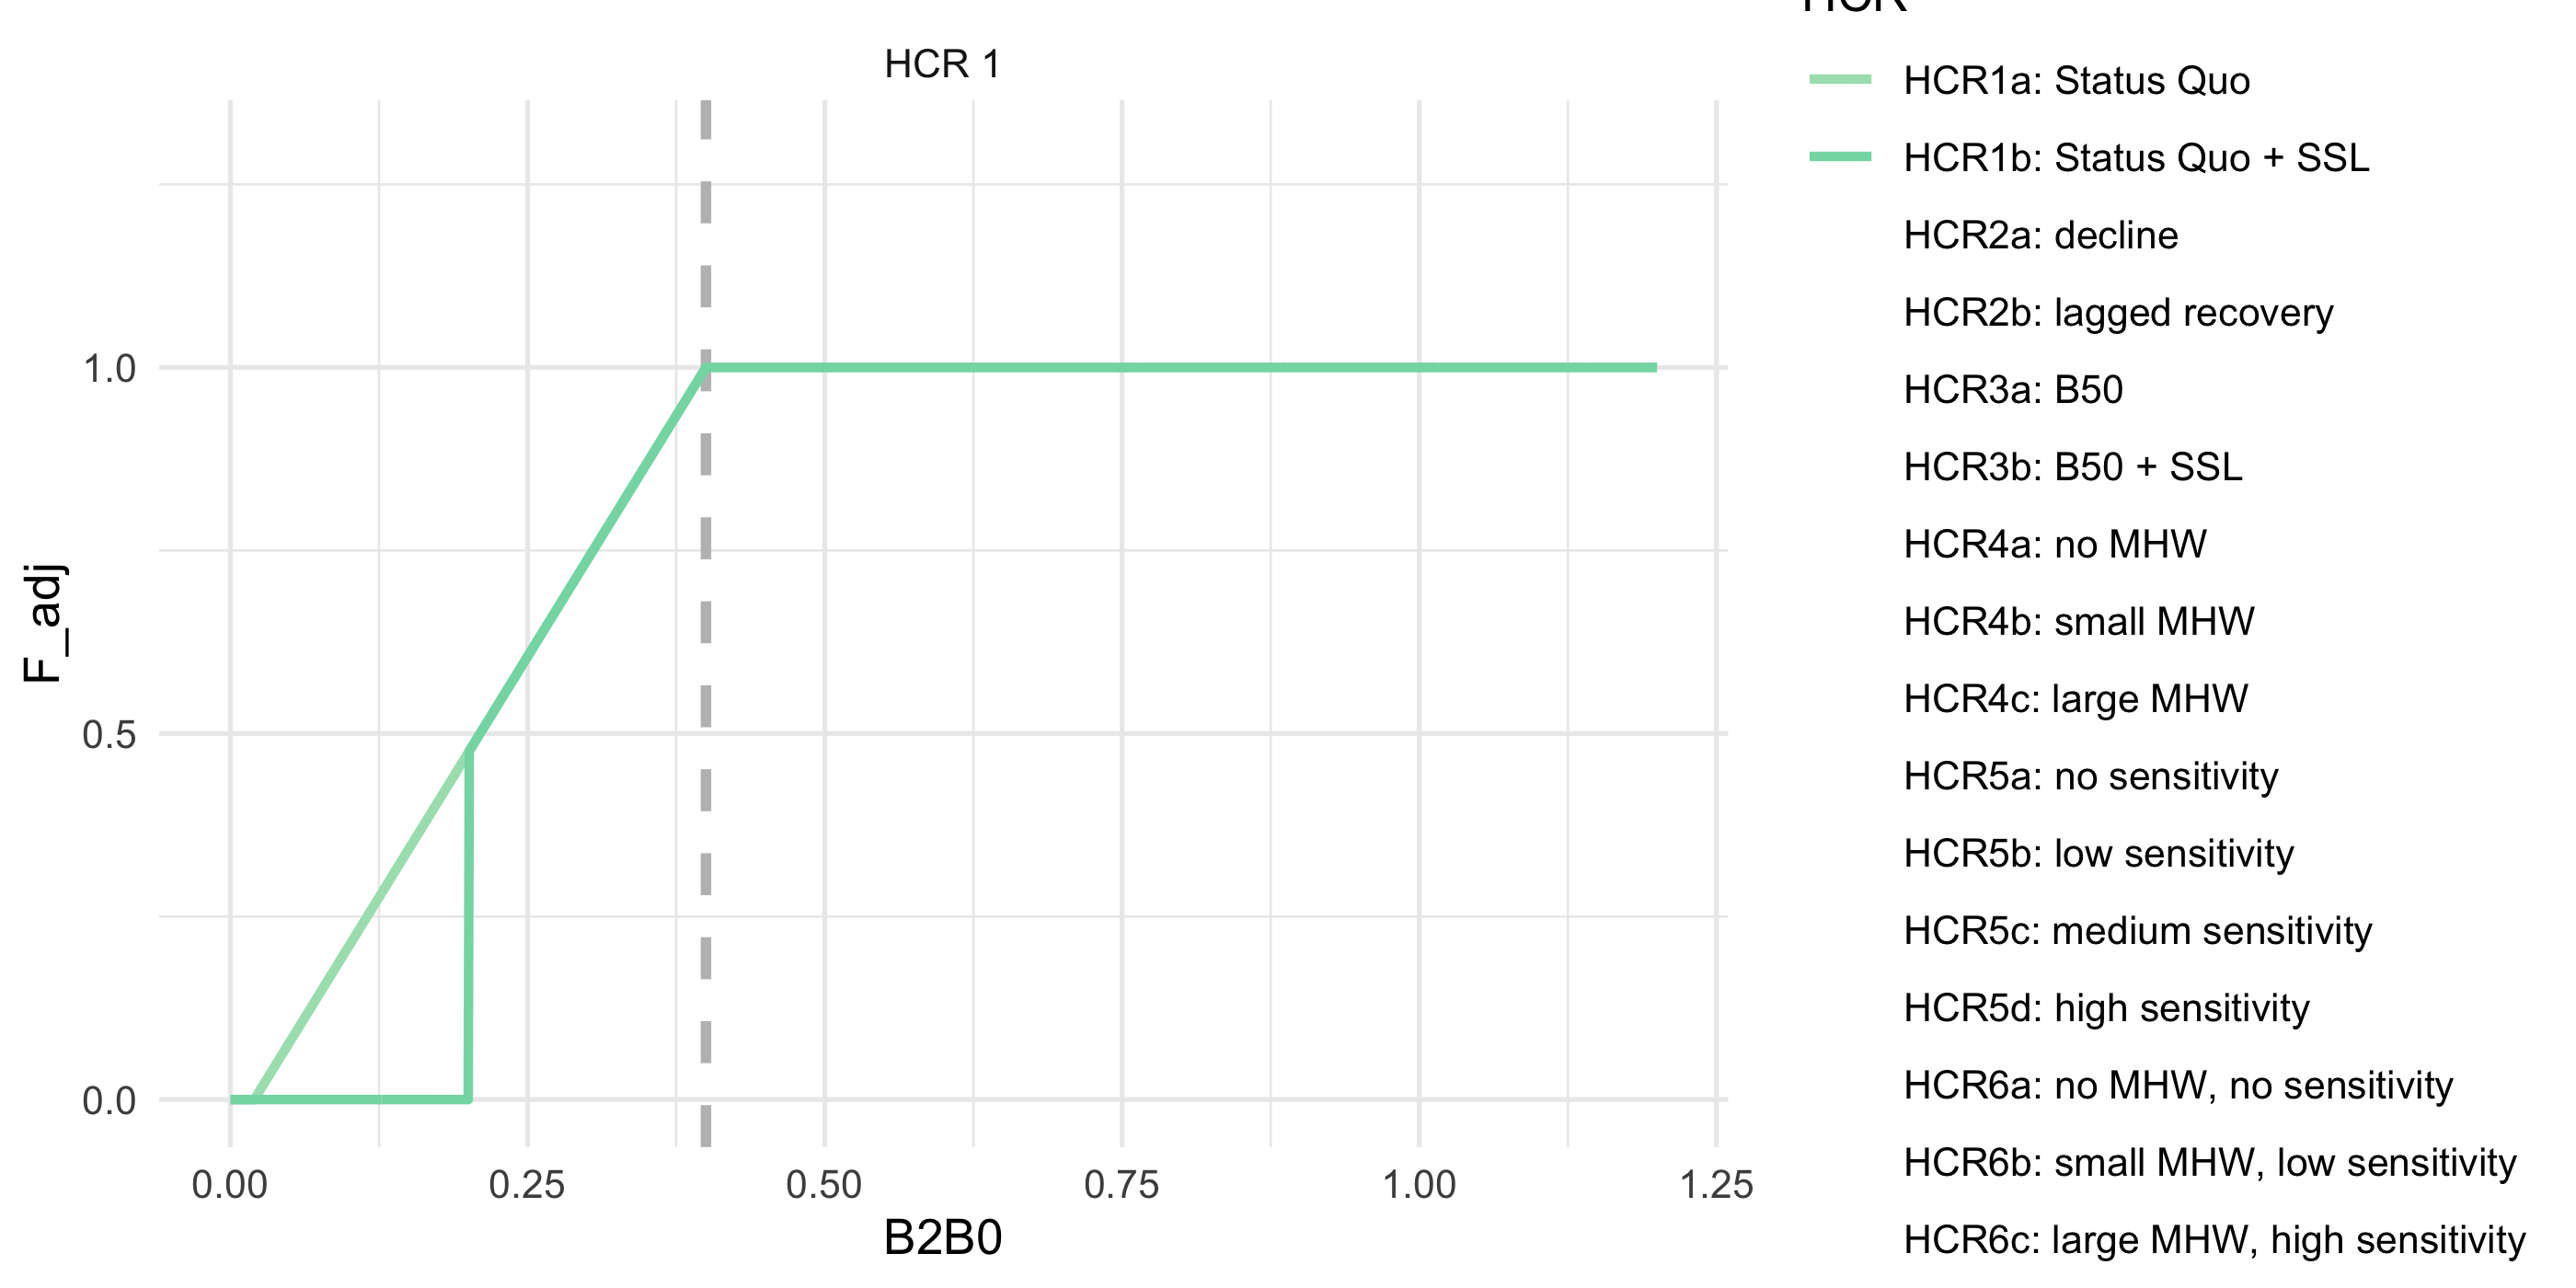
\includegraphics[width=0.8\textwidth,height=\textheight]{../../Figs/HCR_figs/HCR1.png}
\caption{ABC+HCR 1: Status quo. This is the Tier 3 Harvest Control Rule,
including the \(B_{20\%}\) cuttoff for certain species}
\end{figure}

\section{ABC+HCR 2: Lagged recovery to estimate emergency relief
financing
needs}\label{abchcr-2-lagged-recovery-to-estimate-emergency-relief-financing-needs}

This simulation set will help us estimate the approximate cost of
emergency relief funds by artificially closing the fishery at
\(B_{25\%}\)\% (mimicking an enconomic driven closure). During recovery
to mimick lagged fishery recovery from a closure shock, we further delay
F rate by inducing a stronger alpha during the recovery period.
Implementation of this would be to shorten the recovery period following
a shock through a ``rainy day'' fund to supplement the fishery during
climate shocks.

This is the same as in HCR 1 except that the fishery shuts down earlier
at \$B\_\{lim\} = B\_\{25\%\} \$ and during the simulated lagged
recovery the alpha is steeper (slower recovery; \(\alpha = 0.30\)
instead of \(\alpha = 0.05\)

Details: Sloping HCR, \(B_{target} = B_{40\%}\) \(\alpha = 0.05\),
\(B_{lim} = B_{25\%}\), i.e., the cutoff to initiate emergency \$ and a
steeper \(\alpha = 0.30\) during recovery (recovery occurs at
\(B_{40\%}\)). Calculate difference in catch relative to HCR1 to get an
estimate of what \$ relief would be needed to supplement the fishery.
Apply a steeper slope (alpha) on recovery.

Eq. 1 \[F_{ABC_{max}} = \begin{array}{ll}  
 F_{ABC} &~~~~~~~~ \frac{B_y}{B_{target}}>1 \\  
 F_{ABC}((\frac{B_y}{B_{target}}-\hat\alpha_y)/(1-\hat\alpha_y)) &~~~~~~~~ \frac{B_y}{B_{target}} < 1 \leq B_{lim} \\ 
 0 &~~~~~~~~ \frac{B_y}{B_{target}} < B_{lim}  
 \end{array}\]

and,

\[
 \hat\alpha_y =\{ \begin{array}{ll}  
\alpha & if~~\hat\alpha_{y-1} = \alpha ~~|~~ \frac{B_y}{B_{target}} \geq B_{target} \\  
\alpha_{r} &if ~~\hat\alpha_{y-1} = \alpha_{r} ~~|~~ \frac{B_y}{B_{target}} \lt B_{low} \\  
 \end{array}
 \]

For ACLIM HCR2 model runs we set \(\alpha\) to 0.05 and \(\alpha_{r}\)
to 0.3, whith \$ B\_\{low\}\$ = \$ B\_\{lim\}\$ at 0.25.

\begin{figure}
\centering
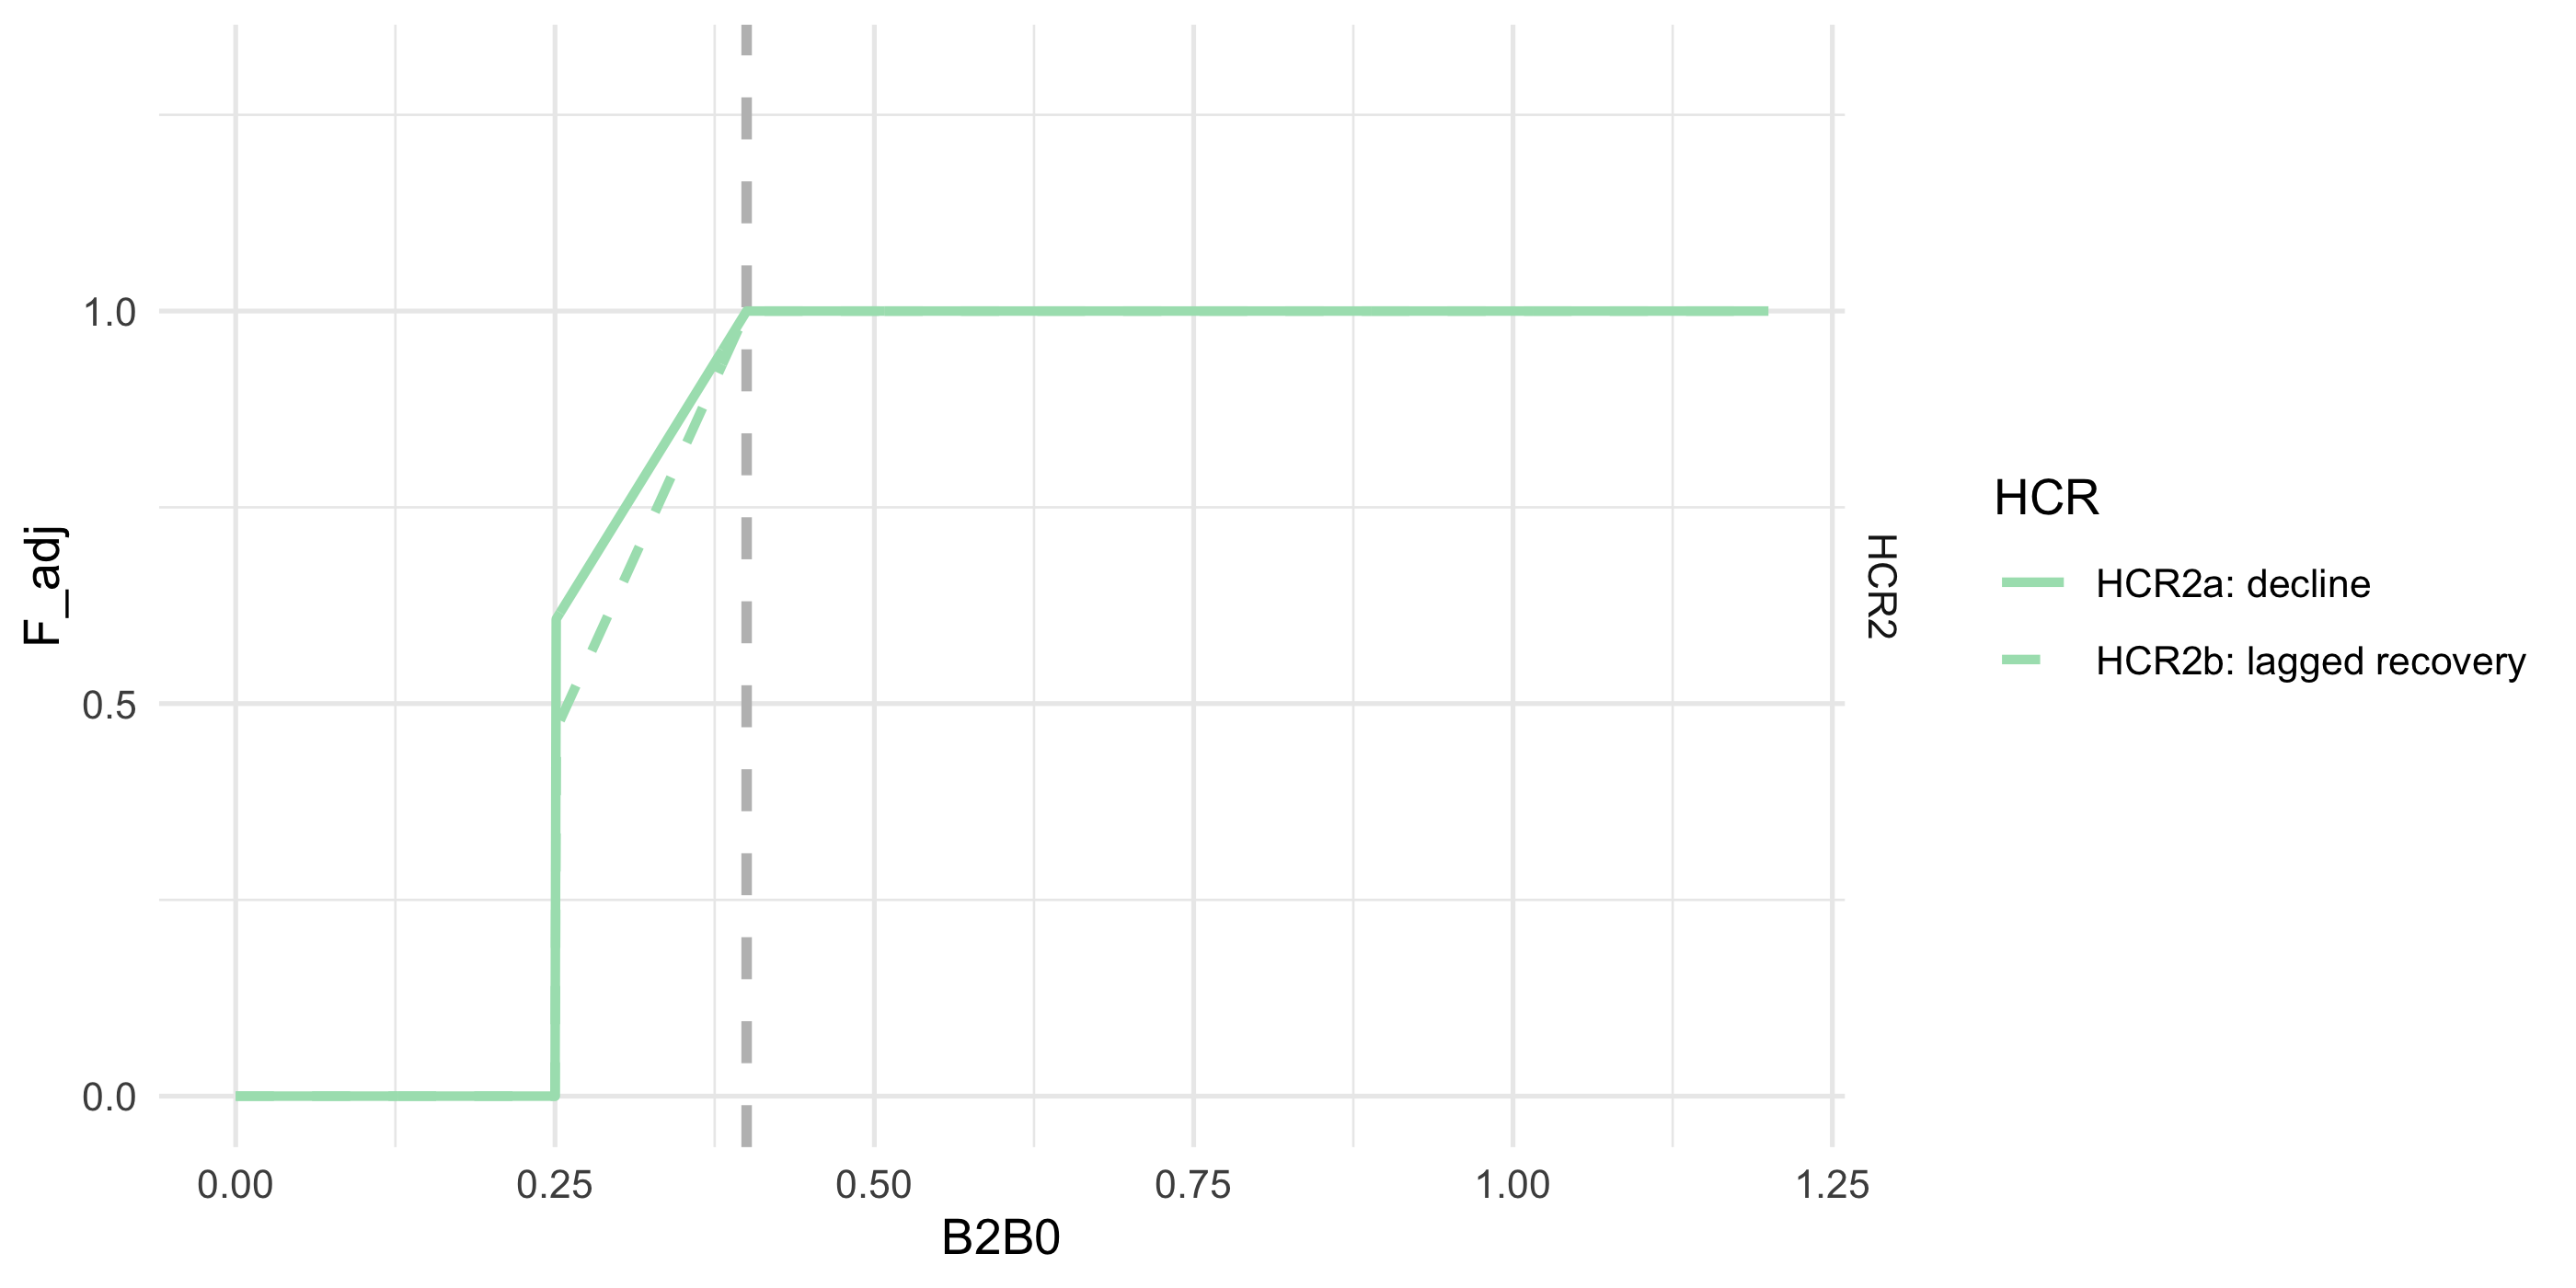
\includegraphics[width=0.8\textwidth,height=\textheight]{../../Figs/HCR_figs/HCR2.png}
\caption{ABC+HCR 2: Lagged recovery to estimate emergency relief
financing needs}
\end{figure}

\section{ABC+HCR 3: Long-term resilience (stronger reserve)
Ftarget}\label{abchcr-3-long-term-resilience-stronger-reserve-ftarget}

This is the same as in HCR 1 except that the fishery shuts down earlier
at \(B_{target} = B_{50\%}\) and during the simulated lagged recovey the
alpha is steeper (slower recovery; \(\alpha = 0.30\) instead of
\(\alpha = 0.05\).

Details: Set the target to 50\% of \(B_{100\%}\) instead of 40\% B40
(\(\alpha = 0.05\), \(B_{lim} = B_{20\%}\), \(B_{target} = B_{50\%}\)).
We're testing whether this would result in more stable biomass levels
and catches.

\begin{figure}
\centering
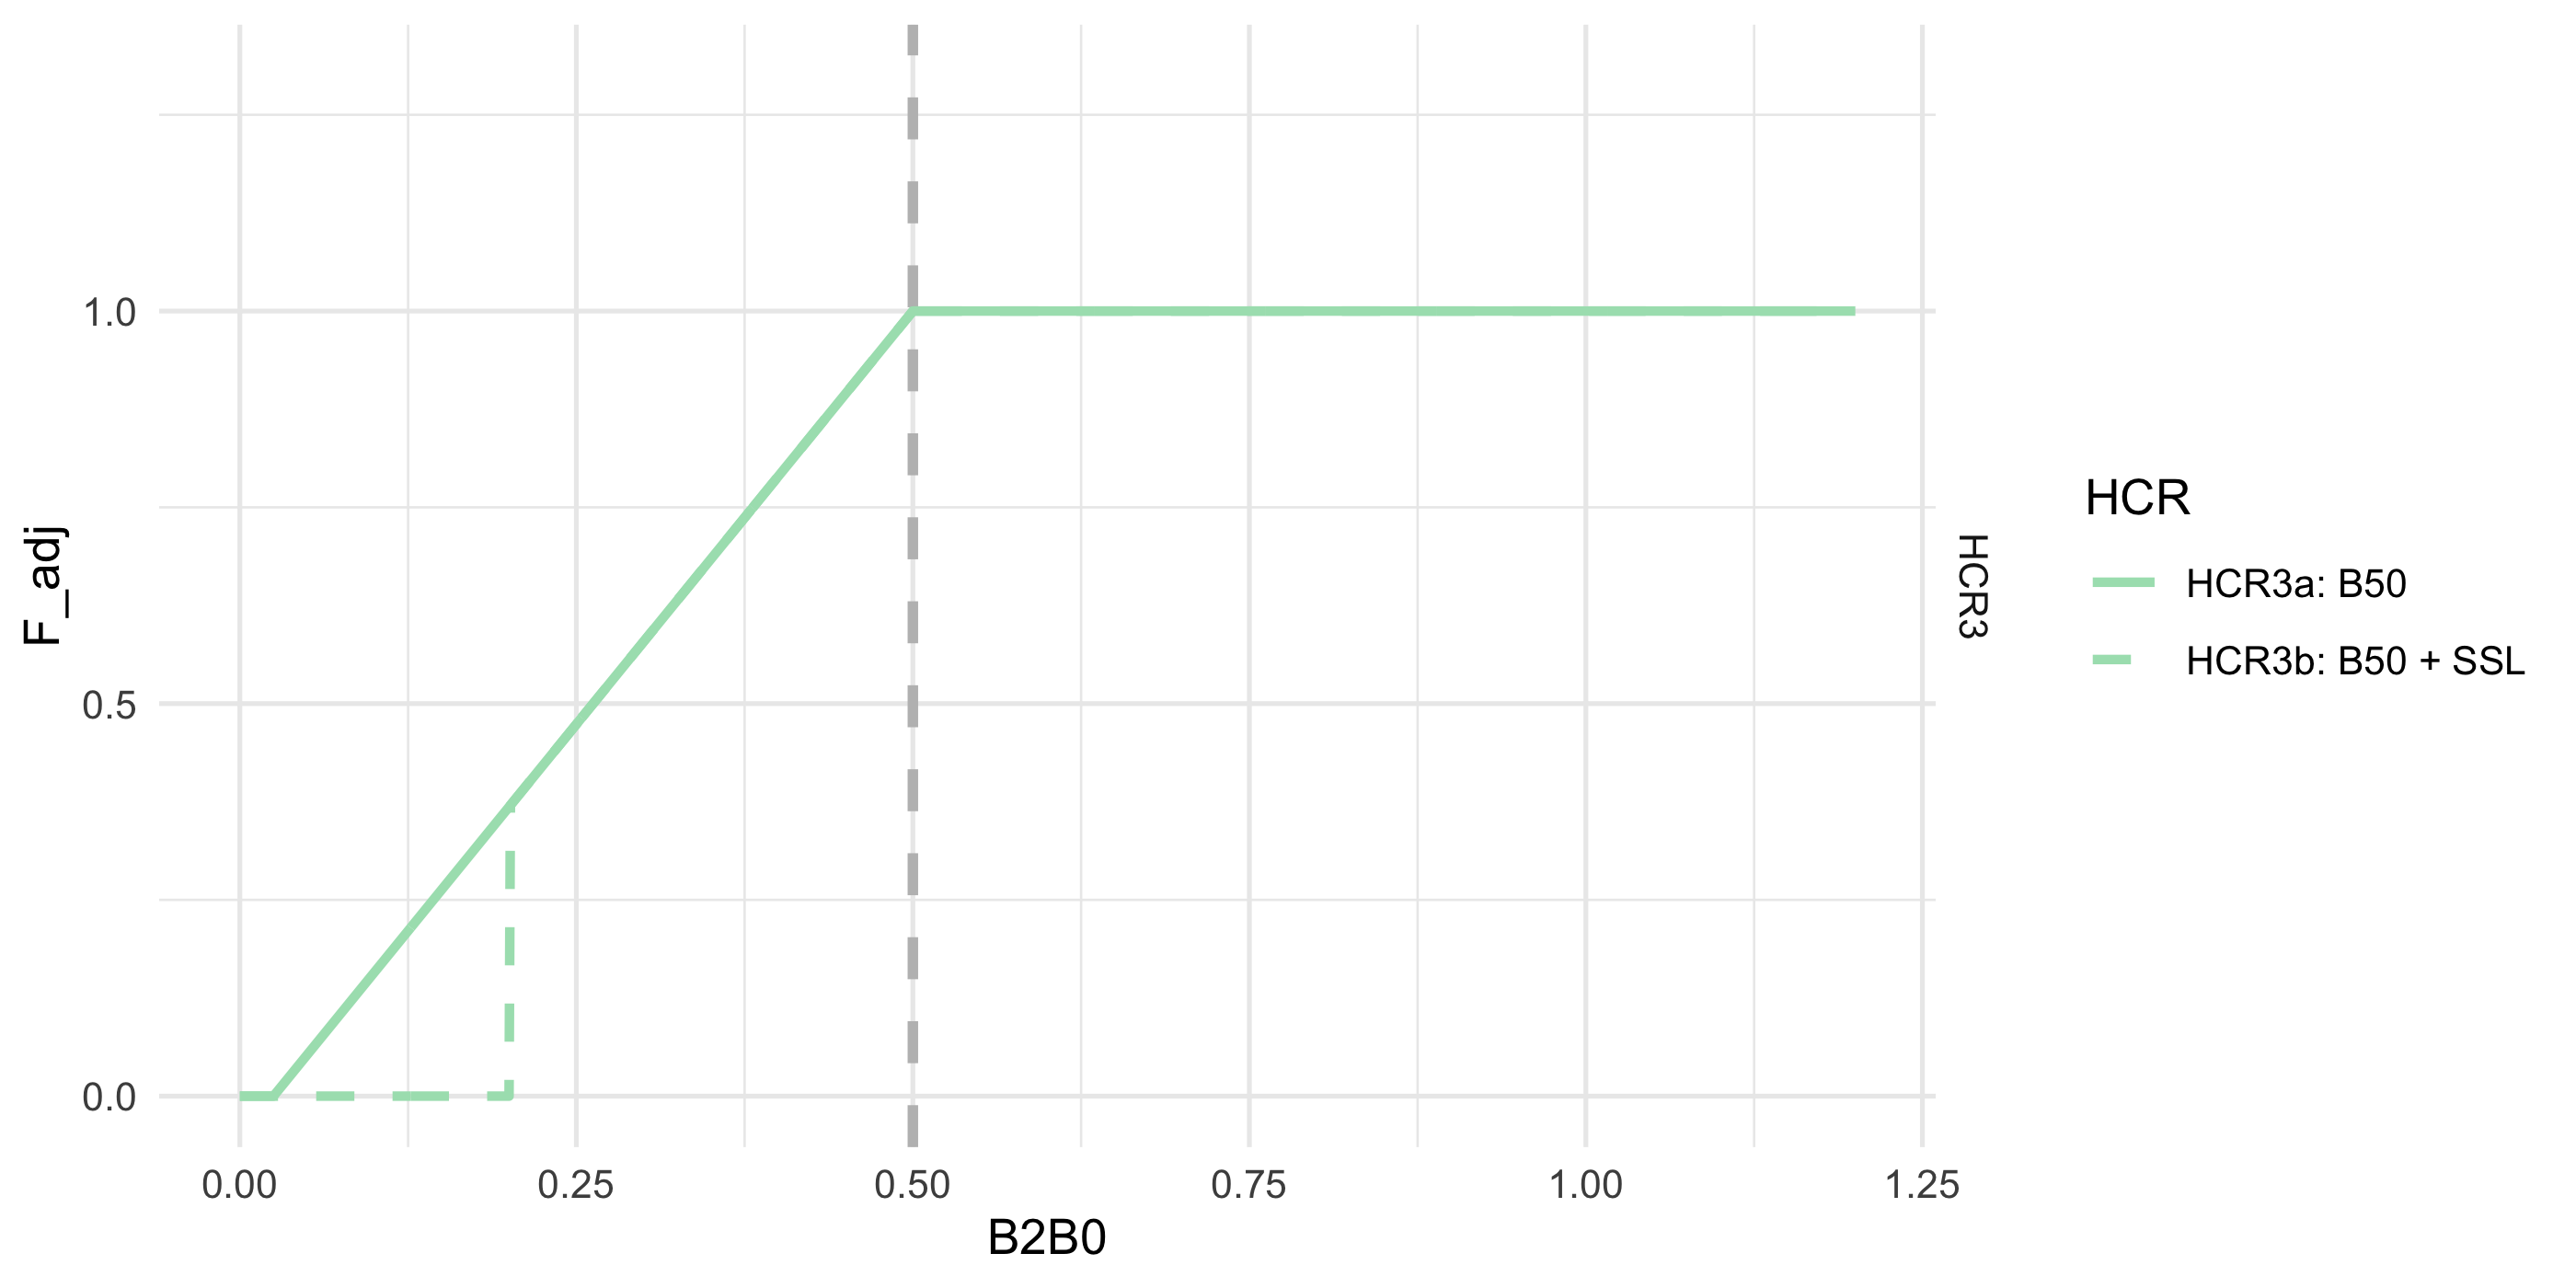
\includegraphics[width=0.8\textwidth,height=\textheight]{../../Figs/HCR_figs/HCR3.png}
\caption{ABC+HCR 3: Long-term resilience (stronger reserve) Ftarget}
\end{figure}

\section{ABC+HCR 4: CE informed sloping rate, e.g., MHW category
alpha}\label{abchcr-4-ce-informed-sloping-rate-e.g.-mhw-category-alpha}

This is the same as in HCR 1 except that the proposed approach would
scale back harvest rates faster below B\_target for species that are
climate sensitive, or during MHWs. Set the target to 40\% of
B\_\{100\%\} (\(\alpha = 0.05\), \(B_{lim} = B_{20\%}\),
\(B_{target} = B_{40\%}\)) for normal conditions/climate resilient
species. But for other species, Below \(B_{40\%}\) have steeper alphas
based on MHW category forecasts for summer conditions ( or
alternatively, climate vulnerability ratings). This reduces future
harvest intensity when conditions are forecast to be poor and could help
rebound stocks faster following MHW. MHWs are characterized as Category
1-4 based on the degree of anomalous conditions above mean climatology
(Category 1 = +1 standard deviations above the mean climatology,
Category 4 = +4 SD).

Details: Set the target to 40\% of \(B_{100\%}\),
(\(\alpha = 0.05+\mathrm{MHW}_{category}*.09\), \(B_{lim} = B_{20\%}\),
\(B_{target} = B_{40\%}\)). E.g., shown, Category 2 MHW set the
\(\alpha = 0.23\), for large MHW set the \(\alpha = 0.41\). We're
testing whether this would result in more stable biomass levels and
catches.

\begin{figure}
\centering
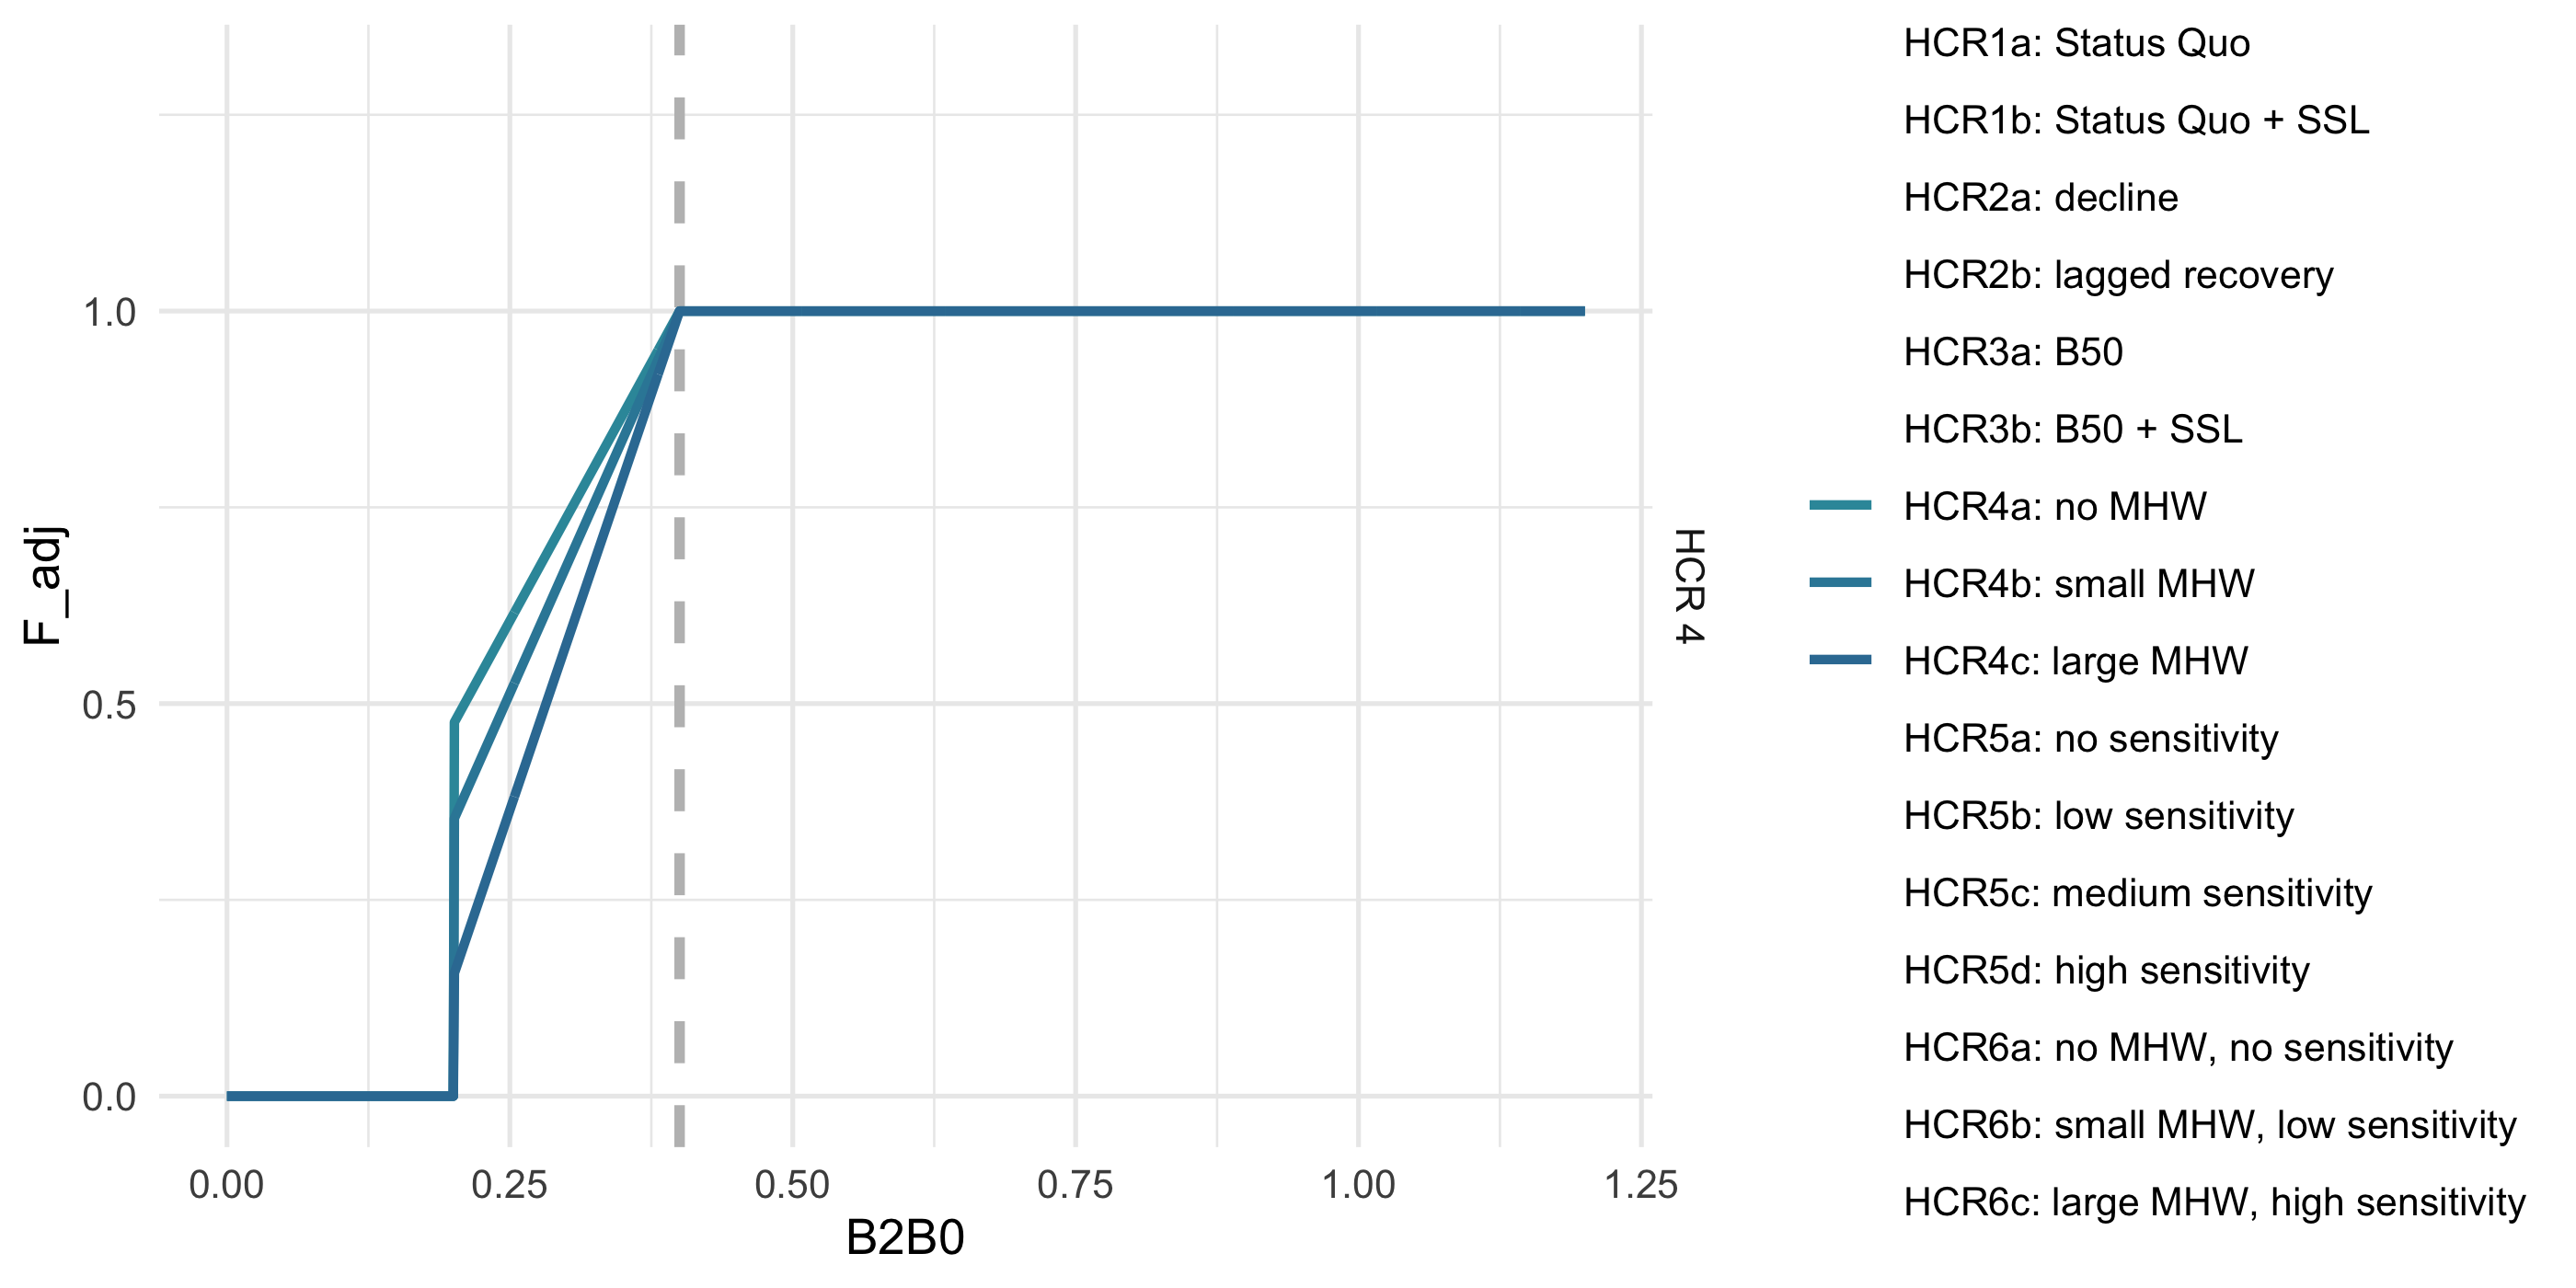
\includegraphics[width=0.8\textwidth,height=\textheight]{../../Figs/HCR_figs/HCR4.png}
\caption{ABC+HCR 4: CE informed sloping rate, e.g., MHW category alpha}
\end{figure}

\section{ABC+HCR 5: climate sensitivity reserve (buffer
shocks)}\label{abchcr-5-climate-sensitivity-reserve-buffer-shocks}

\begin{figure}
\centering
\includegraphics[width=0.85\textwidth,height=\textheight]{../../Figs/Holsmanetal2020_effectiveF.jpg}
\caption{Holsman et al.~2020 Figure}
\end{figure}

The general idea here is to combine the HCR 4 MHW category 0-4 scaling
factor when below B\_target (B40) and a cap-like effect when over
\(B_{target}\) The steepness of that cap effect could be varied based on
vulnerability (or approximated via MSE), more sensitive species might
need more reserve in the ``bank''. Pollock are an example of the HCR 5
in practice (via effects of the 2MT cap + sloping HCR).

Details: Set the target to 40\% of \(B_{100\%}\) (\(\alpha = 0.05\),
\(B_{lim} = B_{20\%}\), \(B_{target} = B_{40\%}\)).After \(B_{40\%}\)
have a slowly sloping F proportional to climate vulnerability (or MHW
category) to mimic realized F rates of pollock under the 2 MT cap, i.e.,
reserve biomass for climate shocks sensu Holsman et al.~2020. This could
use MHW decadal predictions to set the right hand side of the curve
above \(B_{40\%}\).In this the climate sensitivitiy buffer \(\gamma\) is
a value 0 to 1 that scales the reserve for biomass above \(B_{target}\),
i.e., \(B_{40\%}\):

Eq. 1 \[F_{ABC_{max}} = \begin{array}{lll}  
 F_{ABC}\ e^{(-\gamma(\frac{B_y}{B_{target}}-1))} &~~~~~~~~\frac{B_y}{B_{target}}>1, ~~\mathrm{and}~~ \gamma < \frac{B_y}{B_{target}}\\ 
 F_{ABC}((\frac{B_y}{B_{target}}-\alpha)/(1-\alpha)) &~~~~~~~~ \frac{B_y}{B_{target}} < 1 \leq B_{lim} \\  
 0 &~~~~~~~~ \frac{B_y}{B_{target}} < B_{lim}  
 \end{array}
 \]

Details: Set the target to 40\% of \(B_{100\%}\), (\(\alpha = 0.05\),
\(B_{lim} = B_{20\%}\), \(B_{target} = B_{40\%}\)). Shown, for low
sensitivity stocks set \(\gamma = 0.1\), for highly sensitive stocks set
\(\gamma = 0.7\). We're testing whether this would result in more stable
biomass levels and catches through shocks.

\begin{figure}
\centering
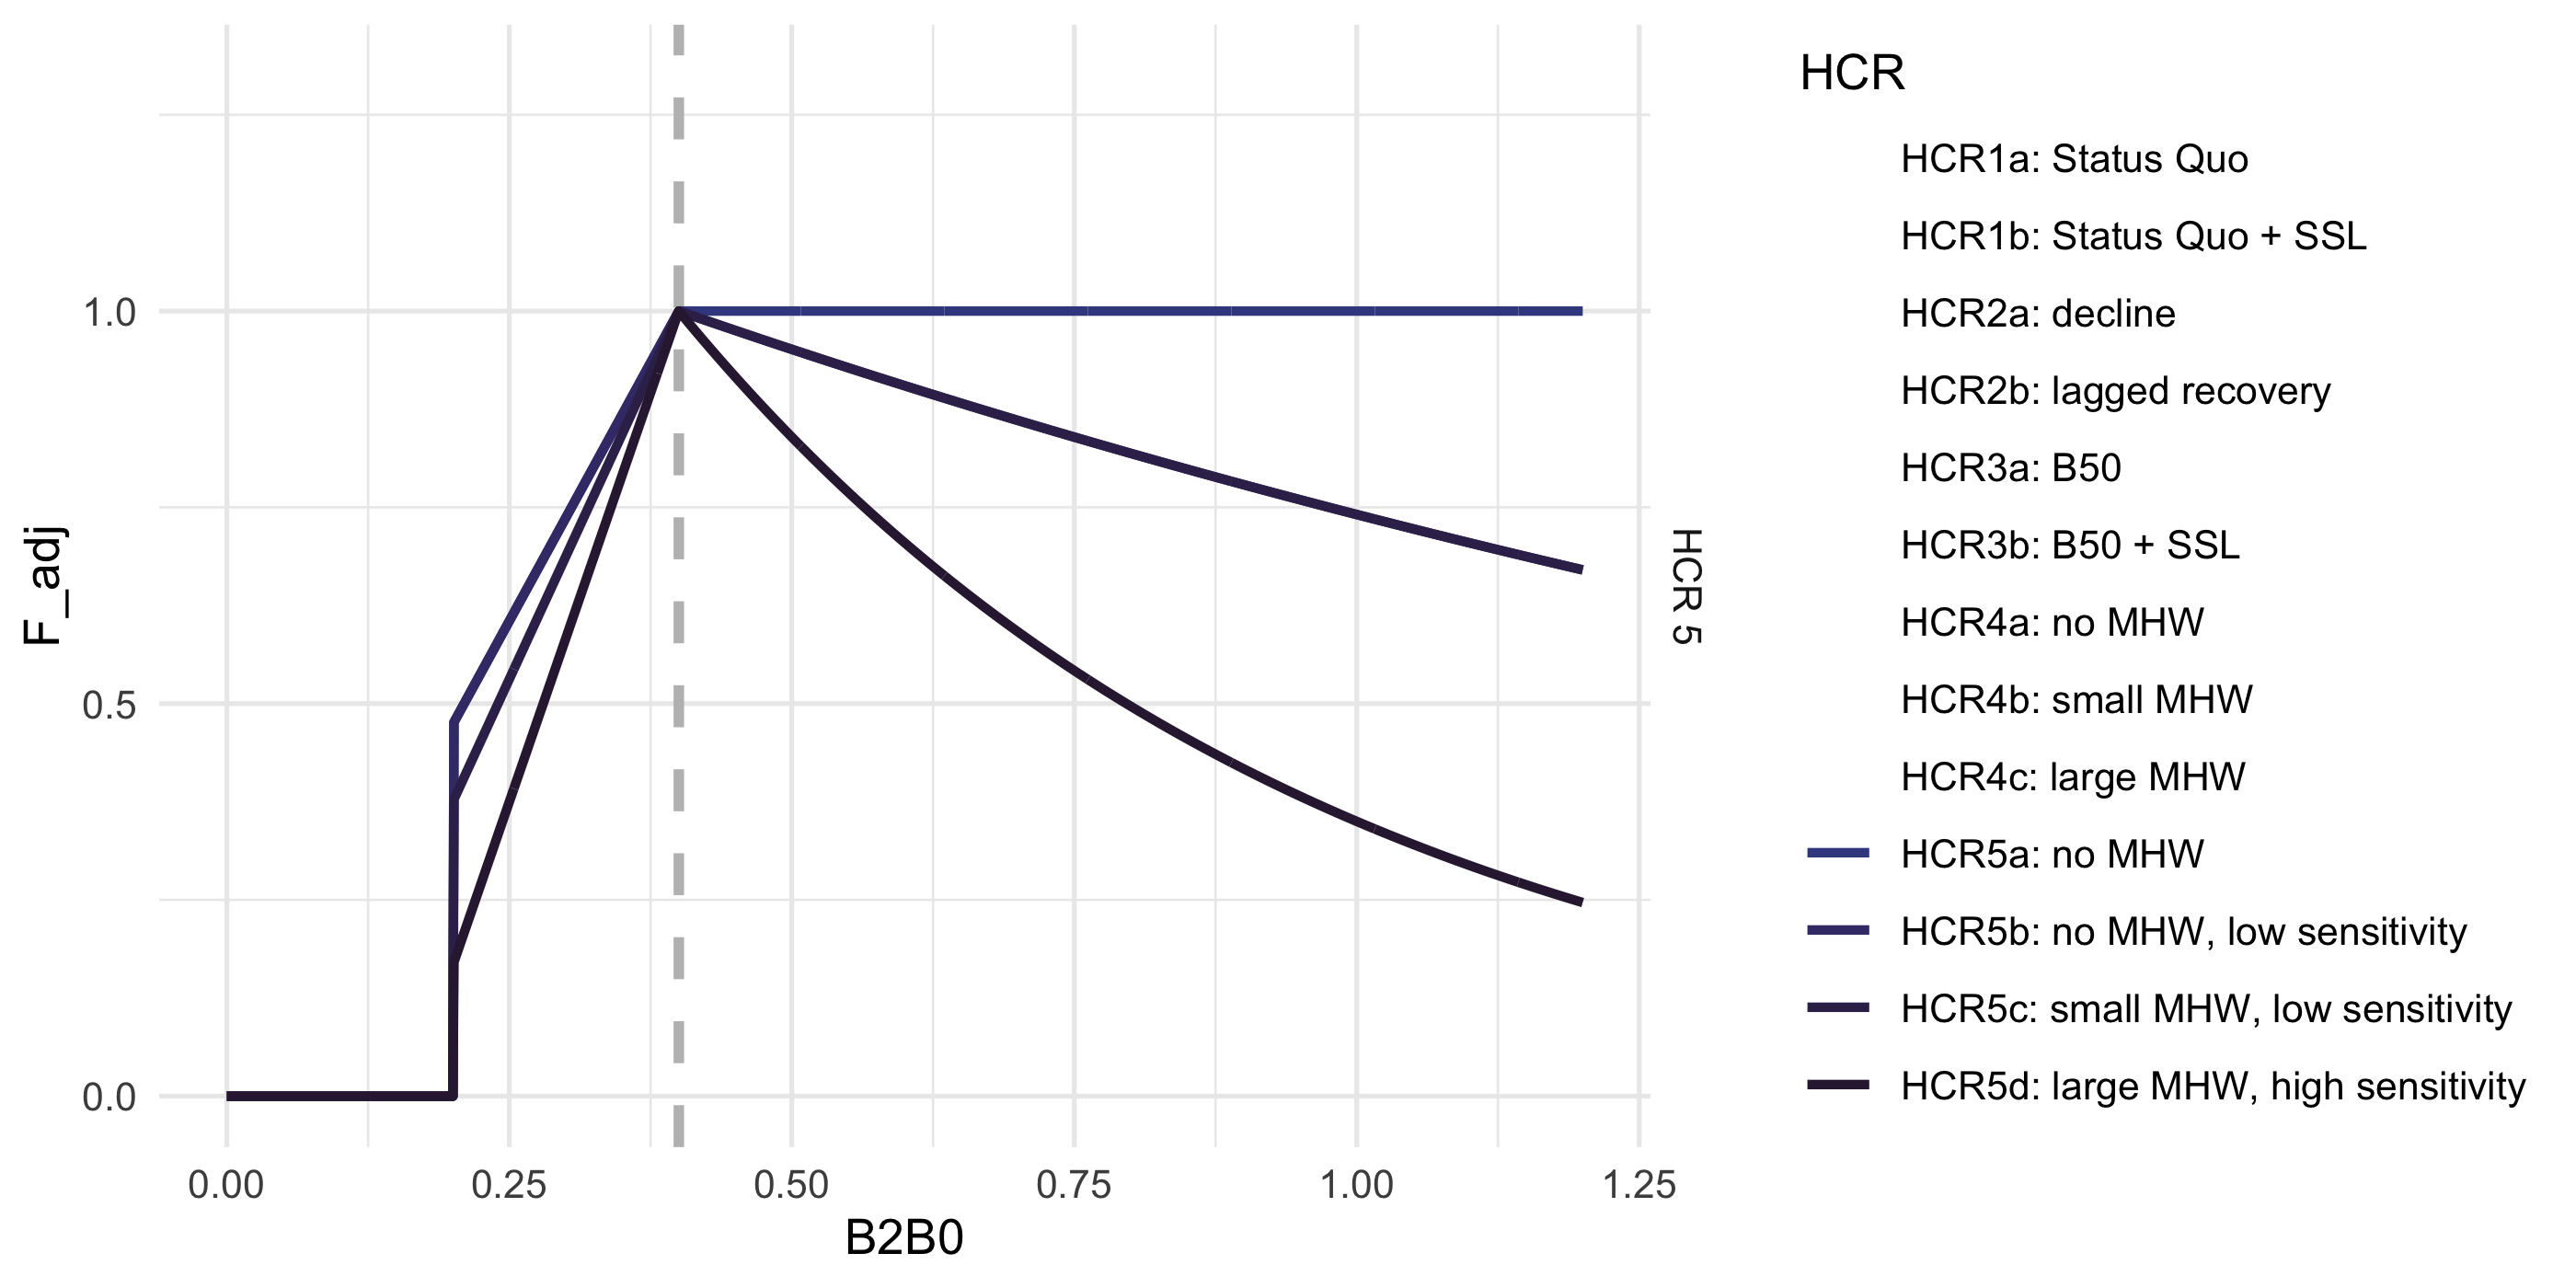
\includegraphics[width=0.8\textwidth,height=\textheight]{../../Figs/HCR_figs/HCR5.png}
\caption{ABC+HCR 5: climate sensitivity reserve (buffer shocks)}
\end{figure}

\section{ABC+HCR 6: MHW slope + climate sensitivity reserve (buffer
shocks)}\label{abchcr-6-mhw-slope-climate-sensitivity-reserve-buffer-shocks}

Here we are exploring the combination of HCR 4 and HCR 5, values are as
specified in those scenarios.

\begin{figure}
\centering
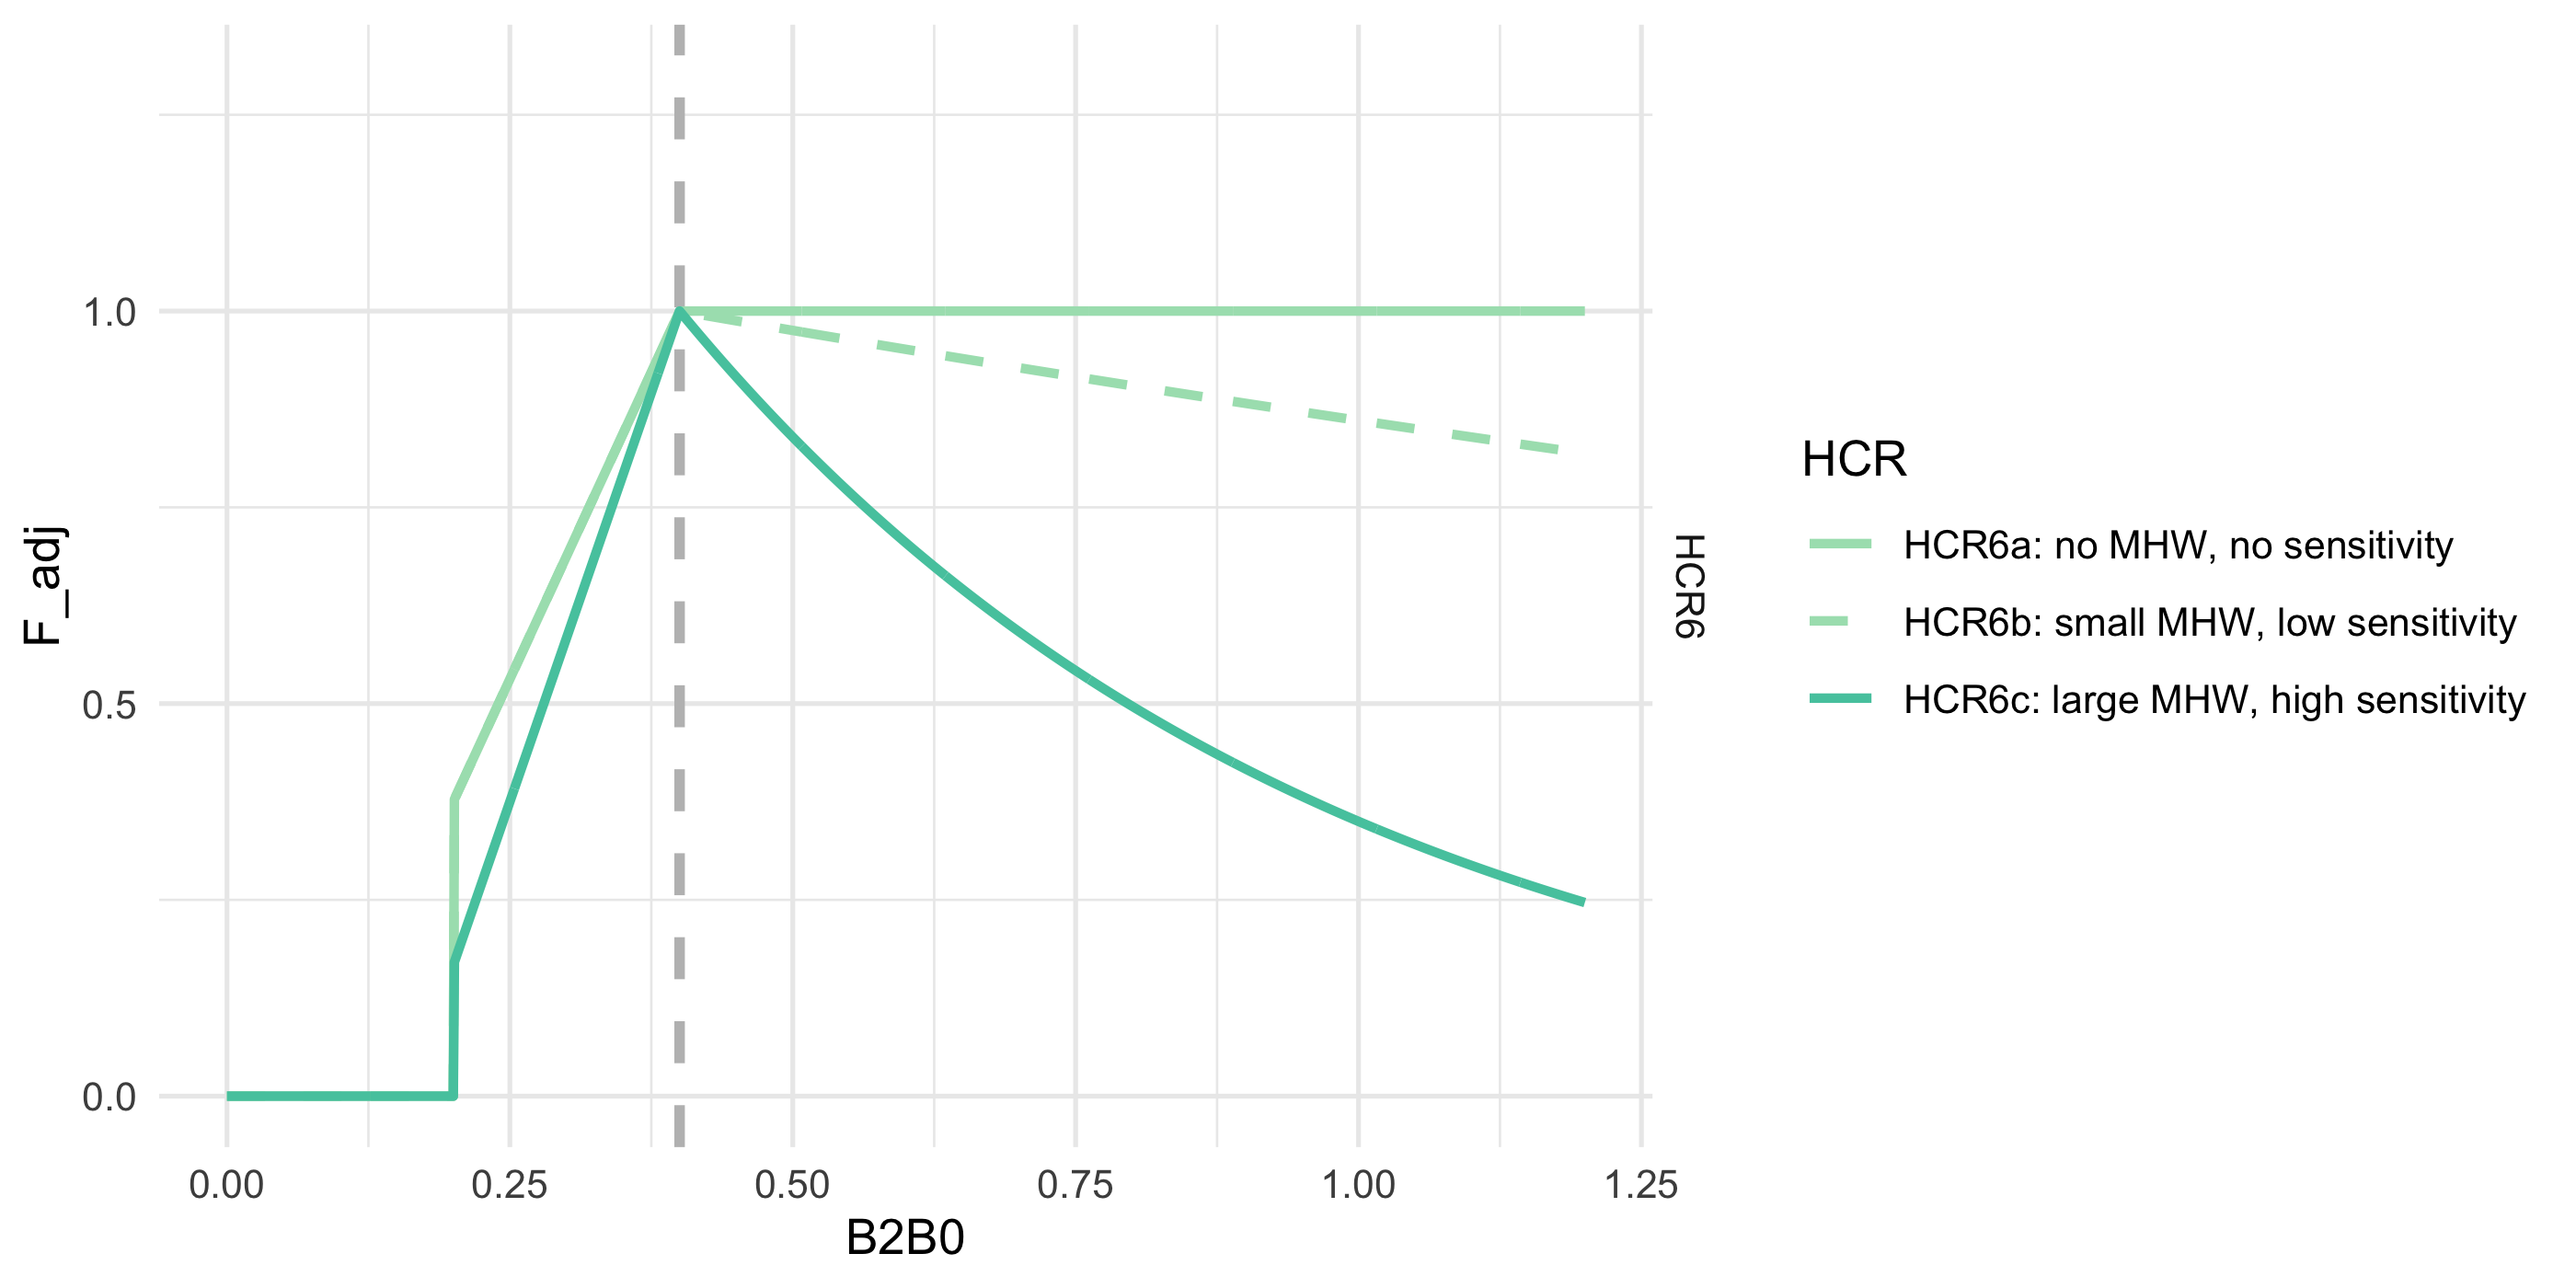
\includegraphics[width=0.8\textwidth,height=\textheight]{../../Figs/HCR_figs/HCR6.png}
\caption{ABC+HCR 6: MHW slope + climate sensitivity reserve (buffer
shocks)}
\end{figure}

\section{ABC+HCR 7:Recruit per spawner biomass variability adjusted HCR
based on analyses by Spencer et al.~in
prep}\label{abchcr-7recruit-per-spawner-biomass-variability-adjusted-hcr-based-on-analyses-by-spencer-et-al.-in-prep}

\[F_{ABC_{max}} = \begin{array}{ll}  
 F_{ABC} &~~~~~~~~ \hat{B}>1 \\  
 F_{ABC}((\hat{B}-\alpha_)/(1-\alpha)) &~~~~~~~~ \hat{B} < 1 \leq B_{lim} \\ 
 0 &~~~~~~~~ \hat{B} < B_{lim}  
 \end{array}\]

where \(F_{ABC}\) is adjusted by covariate \(x_y\) according the
parameter \(\omega_1\) and \(\frac{B_y}{B_{target}}\) is adjusted
basedon the parameter \(\omega_2\) such that:

\[ F_{ABC} =  F_{ABC}e^{(-\omega_1*\mathrm{x_y})}\]\\
and,

\[ \hat{B} = \frac{B_y}{B_{target}}e^{(-\omega_2*\mathrm{x_y})}\]

For the ACLIM HCR 7 simulations \(\omega_1\) and \(\omega_2\) were fit
using retrospecitve analyses of spawner recruitment relationships across
SST (\(x_y\)) on EBS pollock by Spencer et al.~in prep. Values for
\(\omega_1\) and \(\omega_2\) were set to 0.3 and 0.7, respectively.

\begin{figure}
\centering
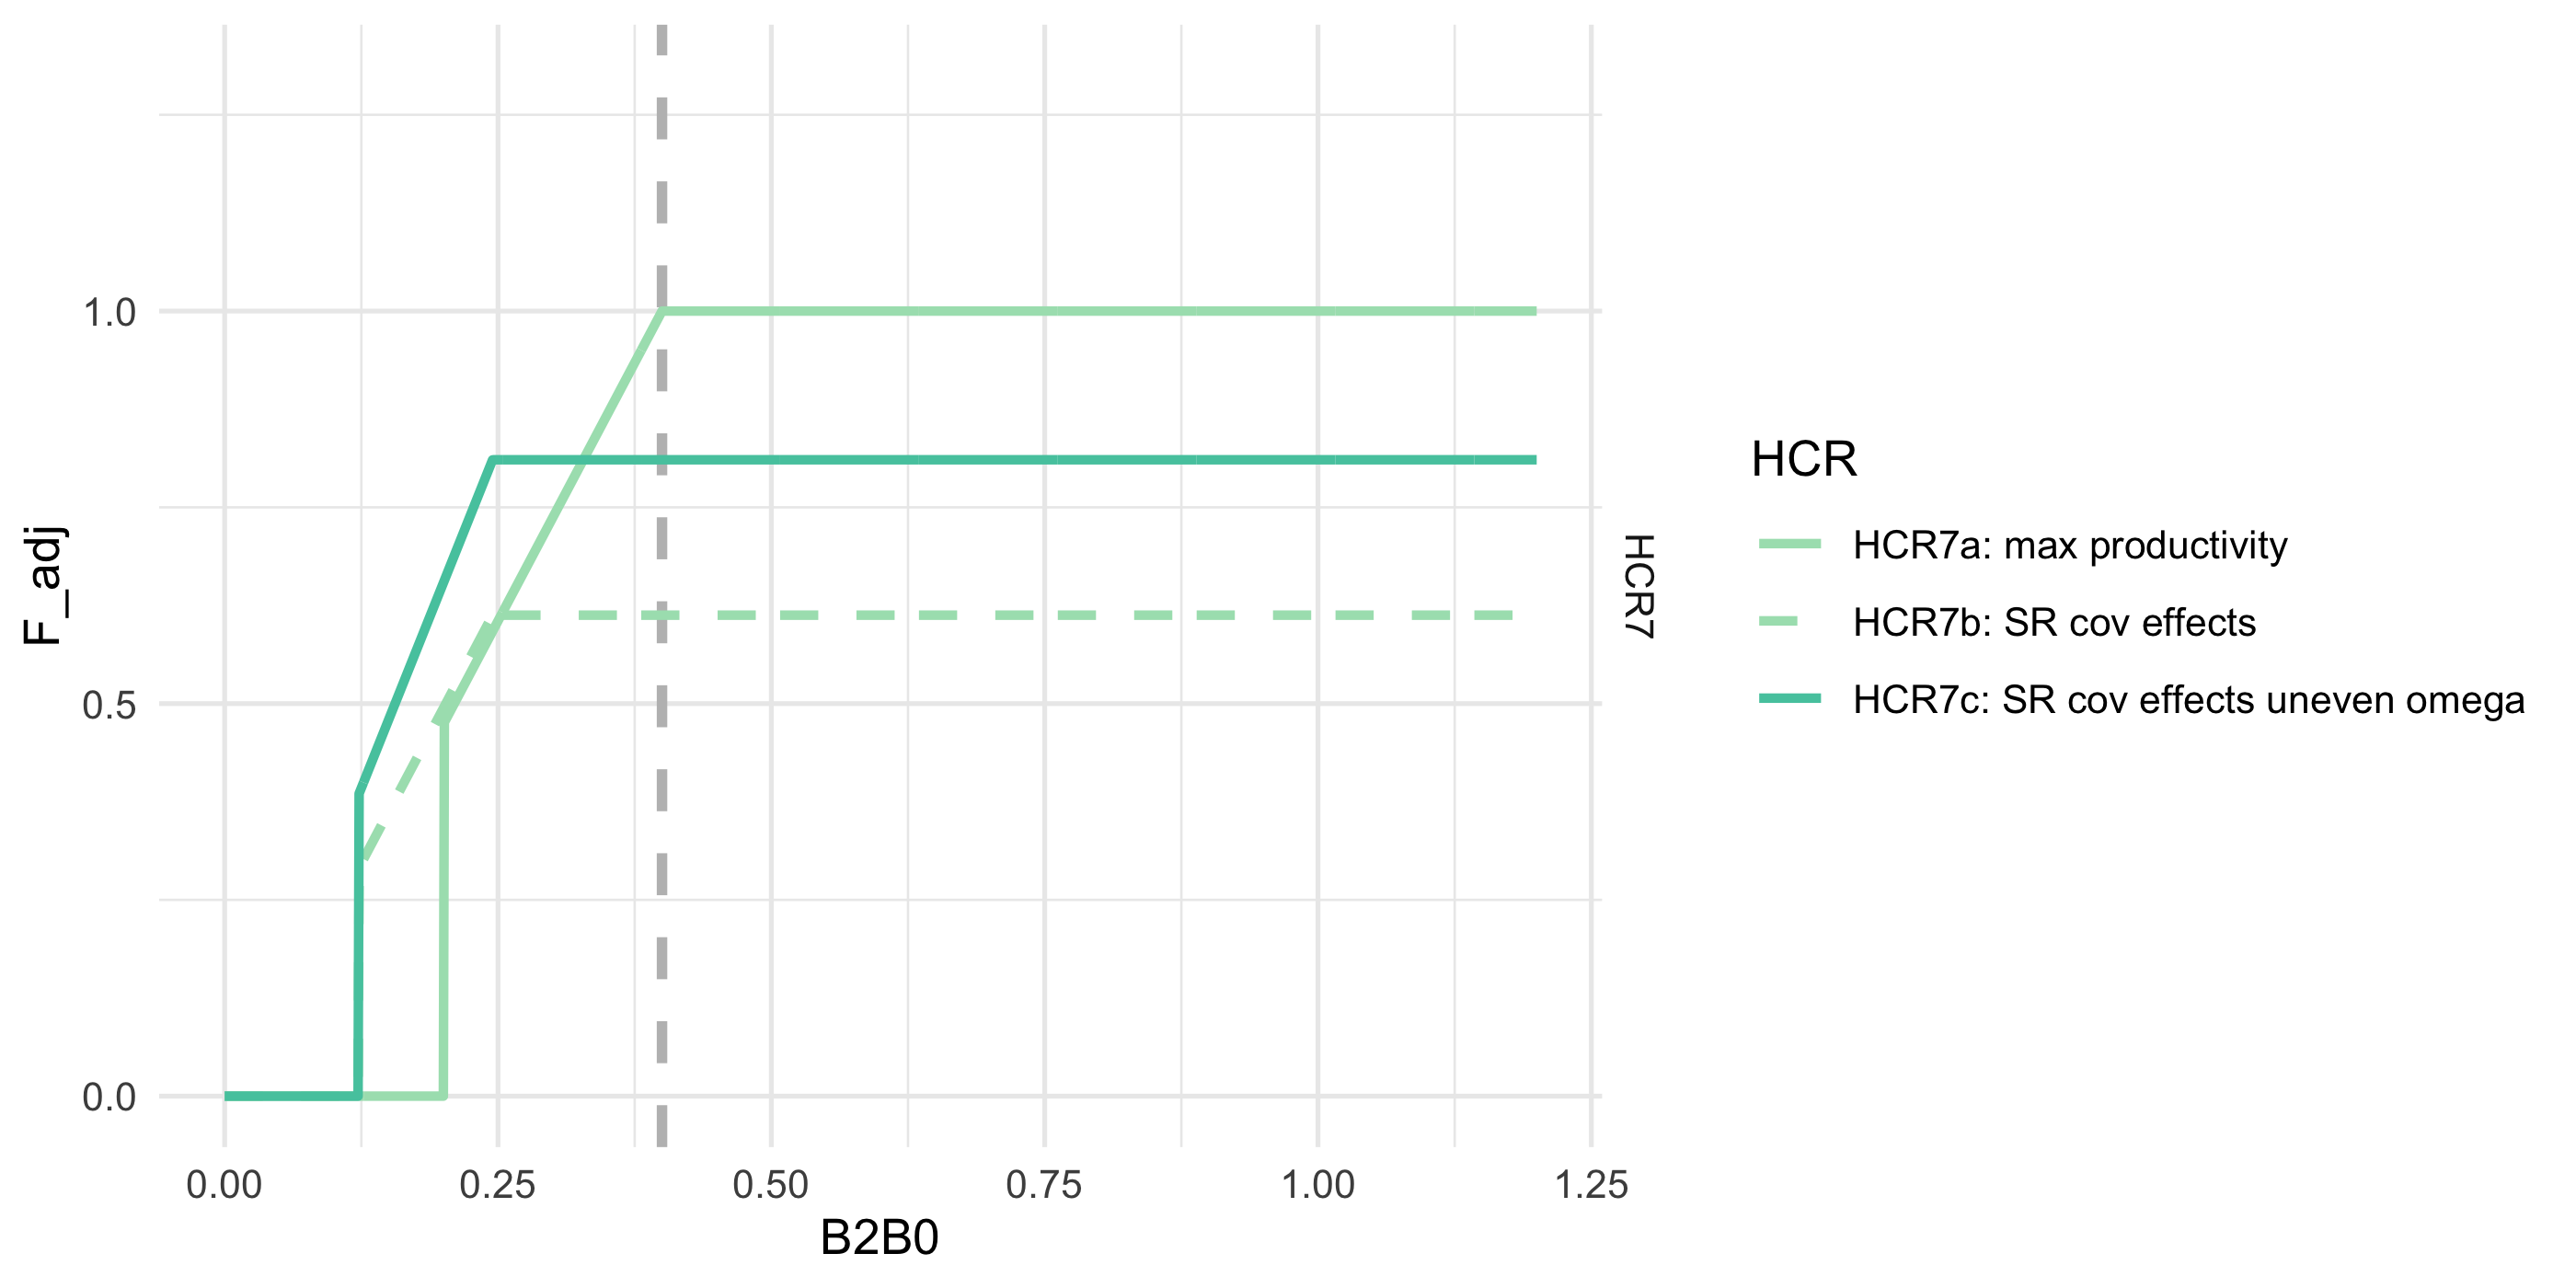
\includegraphics[width=0.8\textwidth,height=\textheight]{../../Figs/HCR_figs/HCR7.png}
\caption{ABC+HCR 7:Recruit per spawner biomass variability adjusted HCR
based on analyses by Spencer et al.}
\end{figure}

\begin{figure}
\centering
\includegraphics[width=0.8\textwidth,height=\textheight]{../../Figs/HCR_figs/HCR1TO6.png}
\caption{ABC+HCR 1- 6: Reserve for rainy day (climate-vulnerability
informed cap effect)}
\end{figure}

\end{document}
